\begin{figure}[t]
\centering
\definecolor{highsucc}{HTML}{66CC66}
\definecolor{midsucc}{HTML}{B9B86A}
\definecolor{lowsucc}{HTML}{F46D6D}
\definecolor{glow}{HTML}{F2F2F2}
\definecolor{ghigh}{HTML}{4A78A8}
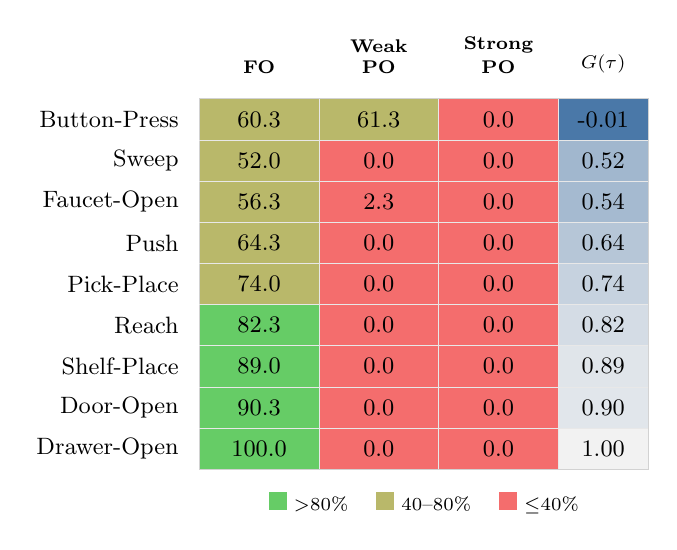
\begin{tikzpicture}[
    scale=0.95, every node/.style={transform shape},
    cell/.style={minimum width=1.6cm, minimum height=0.55cm, font=\small, inner sep=0pt},
    tasklabel/.style={font=\small, anchor=east},
    collabel/.style={font=\scriptsize\bfseries, align=center, anchor=south},
]
\def\cellw{1.6}
\def\cellh{0.55}
\def\gcellw{1.2}

\node[collabel] at (0.5*\cellw, 0.22) {FO};
\node[collabel] at (1.5*\cellw, 0.22) {\shortstack{Weak\\PO}};
\node[collabel] at (2.5*\cellw, 0.22) {\shortstack{Strong\\PO}};
\node[collabel] at (3*\cellw+0.5*\gcellw, 0.22) {$G(\tau)$};

\foreach \row/\task/\fo/\wpo/\spo/\gval in {
    0/Button-Press/60.3/61.3/0.0/-0.01,
    1/Sweep/52.0/0.0/0.0/0.52,
    2/Faucet-Open/56.3/2.3/0.0/0.54,
    3/Push/64.3/0.0/0.0/0.64,
    4/Pick-Place/74.0/0.0/0.0/0.74,
    5/Reach/82.3/0.0/0.0/0.82,
    6/Shelf-Place/89.0/0.0/0.0/0.89,
    7/Door-Open/90.3/0.0/0.0/0.90,
    8/Drawer-Open/100.0/0.0/0.0/1.00} {
    \pgfmathsetmacro{\ypos}{-\row*\cellh-0.5*\cellh}

    \node[tasklabel] at (-0.15, \ypos) {\task};

    \pgfmathtruncatemacro{\fostate}{\fo > 80 ? 2 : (\fo > 40 ? 1 : 0)}
    \ifnum\fostate=2
        \def\focol{highsucc}
    \else\ifnum\fostate=1
        \def\focol{midsucc}
    \else
        \def\focol{lowsucc}
    \fi\fi
    \fill[\focol] (0, \ypos-0.5*\cellh) rectangle +(\cellw, \cellh);
    \node[font=\small] at (0.5*\cellw, \ypos) {\fo};

    \pgfmathtruncatemacro{\wpostate}{\wpo > 80 ? 2 : (\wpo > 40 ? 1 : 0)}
    \ifnum\wpostate=2
        \def\wpocol{highsucc}
    \else\ifnum\wpostate=1
        \def\wpocol{midsucc}
    \else
        \def\wpocol{lowsucc}
    \fi\fi
    \fill[\wpocol] (\cellw, \ypos-0.5*\cellh) rectangle +(\cellw, \cellh);
    \node[font=\small] at (1.5*\cellw, \ypos) {\wpo};

    \pgfmathtruncatemacro{\spostate}{\spo > 80 ? 2 : (\spo > 40 ? 1 : 0)}
    \ifnum\spostate=2
        \def\spocol{highsucc}
    \else\ifnum\spostate=1
        \def\spocol{midsucc}
    \else
        \def\spocol{lowsucc}
    \fi\fi
    \fill[\spocol] (2*\cellw, \ypos-0.5*\cellh) rectangle +(\cellw, \cellh);
    \node[font=\small] at (2.5*\cellw, \ypos) {\spo};

    \pgfmathsetmacro{\gint}{max(0,min(100,100*\gval))}
    \fill[glow!\gint!ghigh] (3*\cellw, \ypos-0.5*\cellh) rectangle +(\gcellw, \cellh);
    \node[font=\small] at (3*\cellw+0.5*\gcellw, \ypos) {\gval};
}

\draw[gray!35, line width=0.3pt] (0, 0) rectangle (3*\cellw+\gcellw, -9*\cellh);
\foreach \i in {1,...,8} {
    \draw[gray!18, line width=0.25pt] (0, -\i*\cellh) -- (3*\cellw+\gcellw, -\i*\cellh);
}
\foreach \x in {\cellw, 2*\cellw, 3*\cellw} {
    \draw[gray!18, line width=0.25pt] (\x, 0) -- (\x, -9*\cellh);
}

\node[font=\scriptsize, anchor=center] at ({(3*\cellw+\gcellw)/2}, {-9*\cellh-0.45}) {
    \tikz{\fill[highsucc] (0,0) rectangle (0.24,0.24);} $>$80\%
    \quad
    \tikz{\fill[midsucc] (0,0) rectangle (0.24,0.24);} 40--80\%
    \quad
    \tikz{\fill[lowsucc] (0,0) rectangle (0.24,0.24);} $\leq$40\%
};
\end{tikzpicture}
\caption{NoMemory success rates (\%) on the 9 MetaWorld tasks under FO, WeakPO, and StrongPO (5 seeds $\times$ 60 episodes). Higher goal-dependency $G(\tau)=S(\mathrm{NM},\tau,\mathrm{FO})-S(\mathrm{NM},\tau,\mathrm{WeakPO})$ tracks larger degradation from FO to WeakPO, while all StrongPO NoMemory scores are 0\%. Button-Press remains nearly goal-independent ($G(\tau)=-0.01$), whereas larger $G(\tau)$ corresponds to progressively larger failure when the goal is hidden. Numeric values are shown in each cell for grayscale readability; darker blue in the $G(\tau)$ column indicates larger goal dependency.}
\label{fig:goal_dependency}
\end{figure}
